\section{Implementación y análisis estadístico de \emph{TRNG} basado en \emph{RO}s}

\subsection{Resumen}

This paper deals with the use of Ring Oscillators (\emph{RO}s) as
pseudo random number generators (\emph{PRNG}).
The design, made for \emph{ALTERA Cyclone} III $^{\copyright} $, using low level primitives is explained.
Two relevant characteristics of a \emph{PRNG} are considered to validate the design: 1) the
equiprobability of all possible outcomes and 2) the statistical
independence of consecutive values. In this work these properties are measured via Information Theory Quantifiers.
A dual entropy plane is used to represent the time series and easily visualize the results obtained with different configurations.
The quality is also compared with other available  \emph{PRNG}s by means of the dual entropy plane.
 Our method constitutes an effective reduction of the complete analysis made with test
suites like \emph{DIEHARD} or \emph{NIST}.

\subsection{Introducción}
\label{sec:Intro}

The jitter and phase noises present in ring oscillators, are not
convenient in several applications of \emph{RO}s, for example in the implementation of \emph{on-chip oscillators} to generate clocks in high-speed circuits\cite{Hajimiri1999,Mandal2010,Gupta2011}. However they are the source of randomness for \emph{RO}-based \emph{PRNG} \cite{Sunar2007,Wold2009}. Furthermore \emph{RO}s can be implemented in a full-digital circuit like Field Programmable Gate Arrays (\emph{FPGA}s) as they  basically are just a string of inverters.


In \cite{Sunar2007}, Sunar et al. presented a \emph{PRNG} using
stochastic jitter by combining several \emph{RO}s. They required a
post processing of the bit stream, based on resilient functions,
to mask imperfections in the entropy source and to increase
immunity against changes in environmental conditions. The entropy of the bit stream was used to
validate the results in \cite{Sunar2007}.


Wold et al. \cite{Wold2009} proposed an enhanced version with
better random characteristics and without a post processing. They only
added an extra D flip-flop at each ring output. The
effectiveness of their proposal was tested by means of test suites available
in the open literature \cite{NIST2000,marsaglia1995,NIST2000a}.

In this paper a detailed description of a very compact hardware implementation of the \emph{RO}-based \emph{PRNG} proposed in \cite{Wold2009} is done.
In order to validate the randomness of the noise sequences generated, two quantifiers derived from the information theory are used. They define a dual entropy plane $H_{BP}$ vs $H_{hist}$.
$H_{hist}$ is a measure of the first characteristic of a \emph{PRNG} pointed in the abstract, the equiprobability among all possible values. $H_{BP}$ is a measure of the second characteristic pointed in the abstract, the independence between consecutive values. This methodology was successful to evaluate randomizing
techniques applied to chaos-based \emph{PRNG} \cite{DeMicco2008}. A comparison with other options both physical and algorithmic, proposed in the literature is made showing that, in spite of their simplicity, \emph{RO}  are good candidates as \emph{PRNG}.

Organization of the paper is as follows: section \ref{sec:hardware} describes the
hardware implementation of the \emph{RO}s mapped in
\emph{FPGA} Cyclone III. Section \ref{sec:method} shows how the normalized entropies are
determined (to keep this paper short we do not detail already
published results); \ref{sec:results} presents the
results obtained for different configurations of the same
\emph{PRNG}s proposed in \cite{Wold2009}, and the statistical comparison with other utilized \emph{PPRNG}s.
Finally we present our conclusions in Sec. \ref{sec:conclusions}.


\subsection{Implementación en Hardware}
\label{sec:hardware}

The implemented \emph{PRNG}'s consist of  several \emph{RO}s
with their outputs XORed together and sampled by a \emph{D} flip flop,
The flip flop latches the output at a selected frequency (here $100$MHz)\cite{Wold2009}.
The physical implementation is made on \emph{ALTERA}$^{\copyright}$  \emph{Cyclone} III \emph{EP3C120}
development kit with a \emph{EP3C120F780C7N} \emph{FPGA}. The design is made with \emph{Quartus}$^{\copyright}$  II 13.1 software.

\subsubsection{Reseña del Chip}

\emph{FPGA}s consist of a large number of logic array blocks (\emph{LAB}s), with groups of logic elements (\emph{LE}s) for implementing sequential as well as
combinatorial circuits. In the \emph{Cyclone} III family architecture
each \emph{LAB} contains $16$ \emph{LE}s.
Basically, each \emph{LE} is a Flip Flop (\emph{FF}) with a
four-input look-up table (\emph{LUT})  (see Fig. \ref{fig:LE}). Each
\emph{LUT} can implement any function of
four variables. The \emph{FF} and the \emph{LUT} can be used together or independently, \cite{Altera}.

%=========================================
 % FIGURA
\begin{figure}
\begin{center}
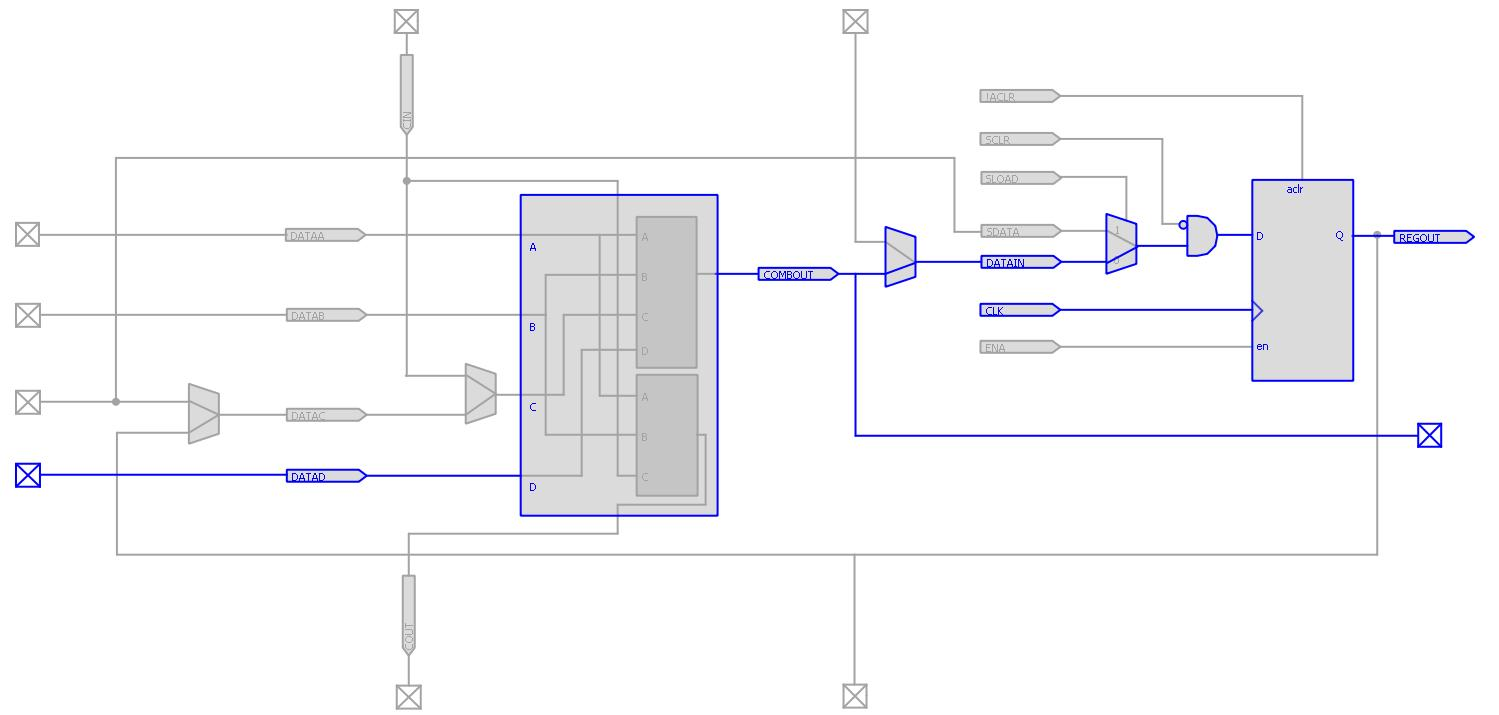
\includegraphics[ width=0.5\textwidth]{NOTenLEmasFF}
\caption{\emph{LE} implementing an inverter and a Flip Flop, Chip Planner
view.} \label{fig:LE}
\end{center}
\end{figure}
%=========================================

Usually, the logic synthesis software assigns \emph{LE}'s
resources without the designer intervention. But in the design of
\emph{RO}-based \emph{PRNG}s it is necessary to control the exact location of
each individual component for two reasons: 1) to avoid the
simplification of the inverters performed by the synthesis tool; 2) to locate
each \emph{RO} in the desired place. In \emph{Altera} the use of low-level primitives enables one to
control the hardware implementation for each \emph{cone of logic} \cite{LowLevel}. Consequently
low-level primitives and assignments are employed inside the \emph{HDL} (hardware description language) code employed in our design.

Strings of \emph{RO}s can be programmed on the chip by
instantiating the \emph{LUT}s as inverters.
In the case of \emph{RO}s it is necessary to prevent the \emph{Quartus} II synthesis engine to merge two \emph{NOT} gates in series, by using a primitive called \emph{LCELL}.
 A \emph{LCELL} always consumes one logic cell and it is not
removed from the project during logic synthesis.

These primitives allow one to break up the design into manageable parts. Each cone is as small as a \emph{LCELL} instantiation.
To create a \emph{RO}, \emph{LCELL}s are programmed as inverter-buffers. Figs. \ref{fig:RTL1ring} and \ref{fig:postMap1ring} show how this primitive is implemented by the Quartus II compiler.

\begin{figure*}
\begin{center}
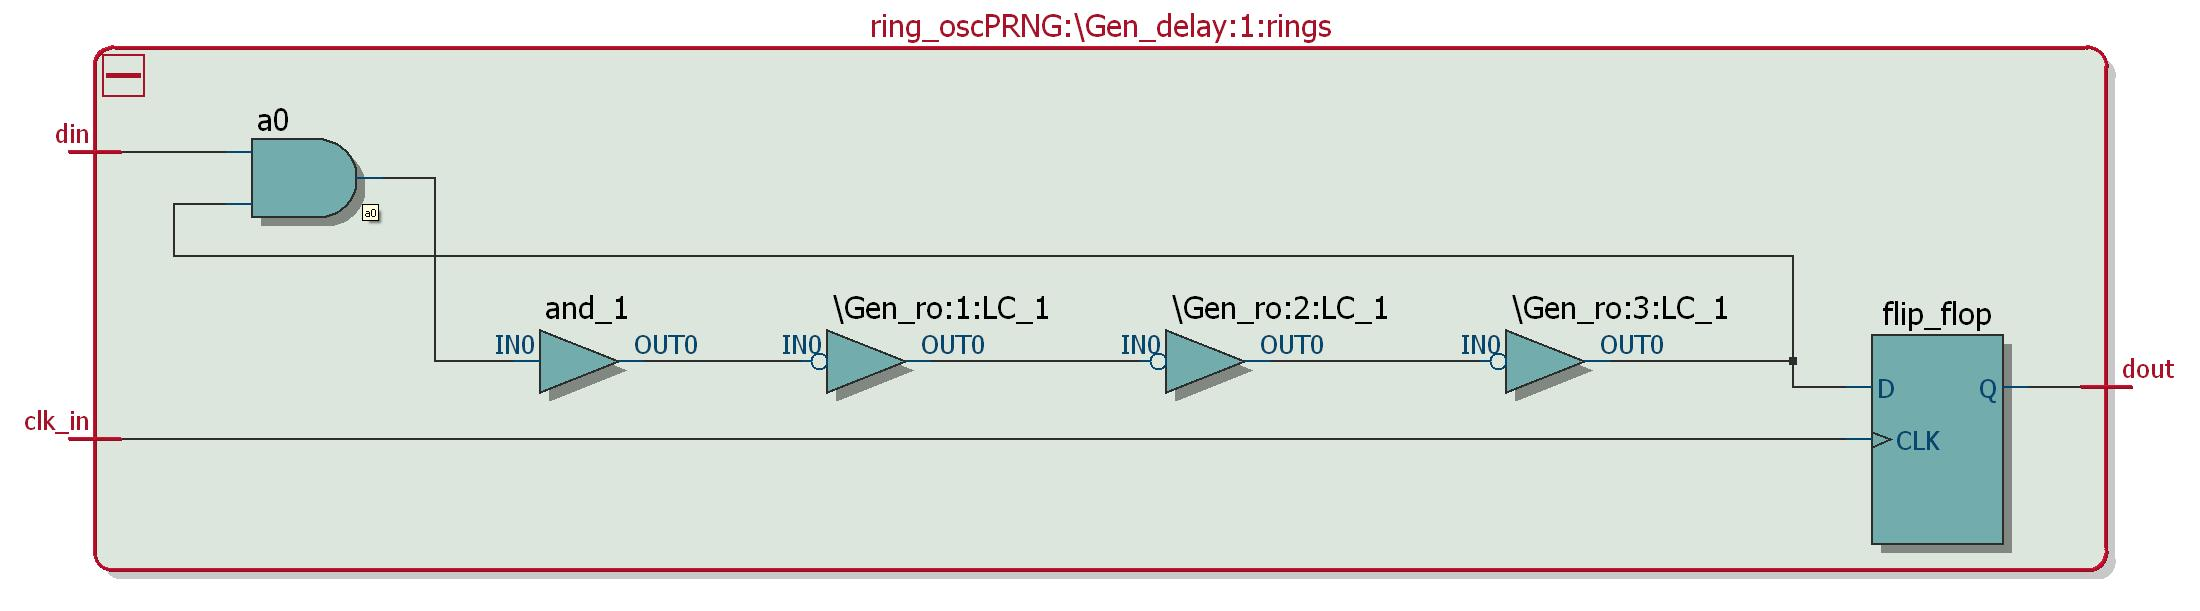
\includegraphics[ width=0.7\textwidth]{RTL_view_1ring}
\caption{RTL view one ring with $3$ inverters.}
\label{fig:RTL1ring}
\end{center}
\end{figure*}

%=========================================
 % FIGURA
\begin{figure*}
\begin{center}
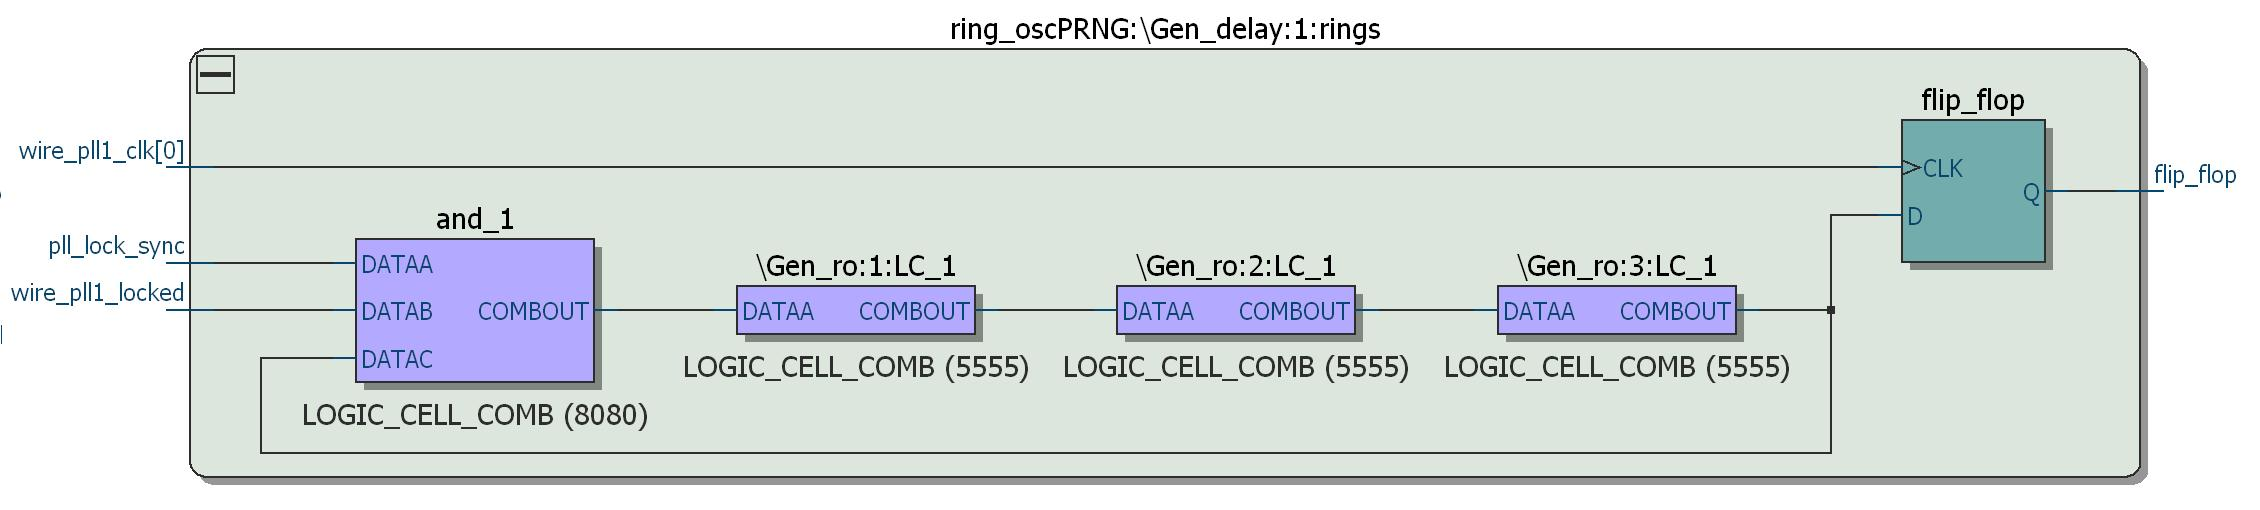
\includegraphics[ width=0.7\textwidth]{tech_map_viewer_post_mapping}
\caption{Technology map viewer (post mapping), one ring with $3$
inverters.} \label{fig:postMap1ring}
\end{center}
\end{figure*}
%=========================================

Furthermore, to avoid the synthesis tool to optimize removing the redundant buffers away,
the \empty{Ignore \emph{LCELL} Buffers} must be set in
\emph{OFF} in the \emph{More Analysis \& Synthesis
Settings} dialog box. Also \emph{Remove Redundant Logic Cells}
must be set to \emph{OFF}.

In order to place each \emph{RO} at a desired position, it
must be assigned to a previously defined \emph{LogicLock region}. In this way the \emph{fitter} will keep all the elements of each ring inside the same region,
\cite{LogicLockRegions}. The process of mapping all the elements to a particular location on the chip
(\emph{LogicLock} region) is achieved by the \emph{Assignment
Editor} tool, that also allows one to verify
that the placements are actually still there, after the  \emph{Synthesis} and \emph{Place \& Route} processes.

Fig. \ref{fig:fpgaplan} shows the $50$ \emph{LogicLock} regions used in this paper as they are
established in the die. One \emph{RO} is assigned to each region.
Regions are spread over the die for a future analysis of location importance. Each region has  $16$ \emph{LAB}s, to allow us to increase the number of inverters of each ring, an issue to be considered in future work.


%=========================================
 % FIGURA
\begin{figure*}
\begin{center}
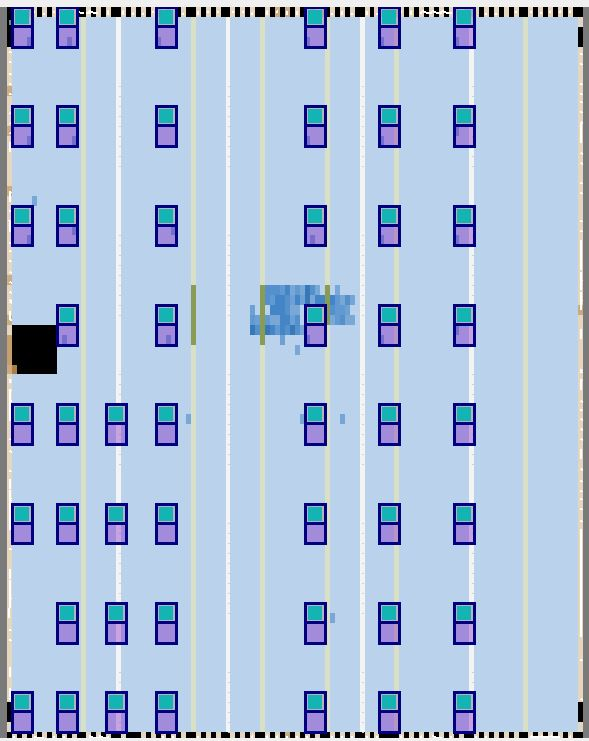
\includegraphics[ width=0.5\textwidth]{fpgaplan}
\caption{\emph{Chip Planner} view \emph{LogicLock} regions.}
\label{fig:fpgaplan}
\end{center}
\end{figure*}
%=========================================

 $3-$inverters, employed in a \emph{RO} and the \emph{FF} were all mapped onto a  \emph{LE} each, meaning that the block
utilization is $4$ of $16$ \emph{LE}s for any \emph{LAB}.


Fig. \ref{fig:LE} displays a single \emph{LE}, there an inverter is
implemented in the \emph{LUT} and it can be seen the exact
\emph{LUT} input that is used. Also the output \emph{FF} of
the ring is mapped there.


There are many factors that determine the frequency of each
\emph{RO}, and contributes to the unpredictability of the output:
\begin{enumerate}
\item Placement within the \emph{LAB}: different placements between rings could result in timing differences.
\item Connections: even having exactly
identical placement of the \emph{LUT}s with respect to each other
in a given ring, it is not possible to have exactly the same
\emph{routing resource usage} in the connections. A small difference in
\emph{routing resource usage} could affect the ring delay.
\item Input selection:  the \emph{fitter} will choose which
\emph{LUT} input is utilized during the routing stage. But the delay through the \emph{LUT}
depends on which of the four inputs is used and consequently the rings could
also have different delays.
\item Neighborhood: even if the design locks down all the placement and routing of a
section  and everything is
physically locked, the timing can change by a few picoseconds
depending on what is placed and routed around the ring.\end{enumerate}
%
In Fig. \ref{fig:RTL3rings} (RTL view) it is shown a \emph{PRNG} using $3$ \emph{RO}s
followed by a XOR gate.

% FIGURA
\begin{figure}
\begin{center}
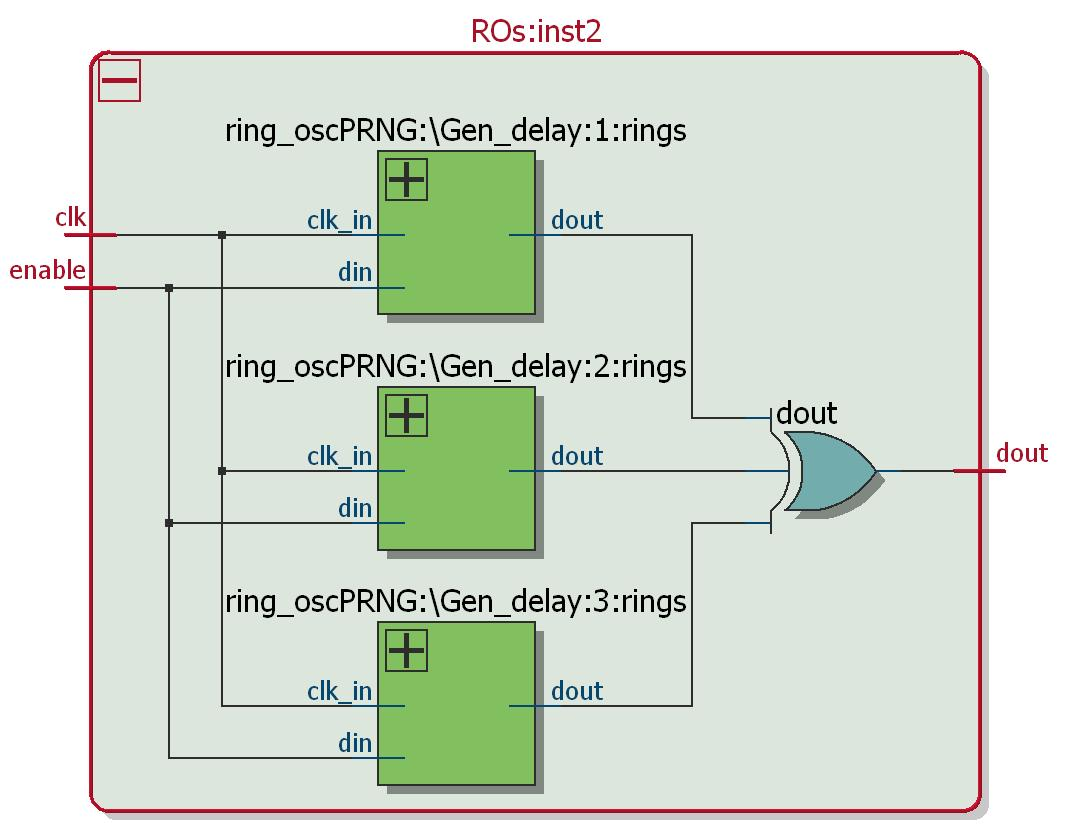
\includegraphics[ width=0.5\textwidth]{RTL_view_3ROs}
\caption{\emph{RTL} view of \emph{PRNG} with $3$ \emph{RO}s.}
\label{fig:RTL3rings}
\end{center}
\end{figure}

%=========================================

Finally, Table \ref{compilation} shows the compilation report of the \emph{PRNG}  using $15$ \emph{RO}s each with $3$ inverters.


%=========================================
\begin{table}
\begin{center}
\begin{tabular}{| l | c  c | }
 \hline
 
\footnotesize{Total logic elements} & $847/119,088$ & $ ( < 1 \%)$\\

 \hline
 
\footnotesize{Total combinational functions} &  $629/119,088$ & $( < 1 \%)$ \\

 \hline
 
\footnotesize{Dedicated logic registers} & $617/119,088$ & $( < 1 \%)$ \\

 \hline
 
\footnotesize{Total registers} &  $617$ &   \\

 \hline
 
\footnotesize{Total memory bits} &  $131,072/3,981,312$ & $( 3 \%)$ \\

 \hline
 
\end{tabular}
\end{center}
\caption{Compilation Report, \emph{RO}-based \emph{PRNG} using $15$ \emph{RO}s and $3$ inverters each.}
\label{compilation}

\end{table}





In this paper we adopt plane $H_{BP}$ vs $H_{hist}$ \cite{DeMicco2008}  to represent each \emph{PRNG}. A higher
value in any of the entropies, $H_{BP}$ and $H_{hist}$, implies an
increase in the uniformity of the involved \emph{PDF}'s. The point
$(1,1)$ represents the ideal point for a \emph{PRNG} with uniform histogram and
uniform distribution of ordering patterns.

\subsection{Resultados}
\label{sec:results}

The  \emph{Embedded Logic Analyzer} tool is utilized for collecting the random sequences generated.
It constitutes a \emph{system-level debugging tool}, provided by $Altera$  \cite{QUARTUS}, that captures and storages the real-time signal behavior and allows one to observe interactions between hardware and software in system designs. After acquiring
the data and  save them into a \emph{SignalTap} II file, they can be
analyzed or viewed as a waveform. With this procedure nor extra jitter neither distortion are introduced in the measured signal from the data acquisition chain.

In the case of \emph{RO} based \emph{PRNG}
data files with $917504$ bits each were generated for each \emph{RO} based \emph{PRNG}.
We consider sets of $N_{RO}$ rings, each with $3$ inverters; $N_{RO}=2$, $3$, $4$, $5$, $6$, $7$, $15$, $25$ and $50$.

Data from $SignalTap$ were  processed using \emph{Matlab}$^\copyright$. Binary data were grouped in $6$-bits words without
superposition, so files with $152917$ data each were generated. Quantifiers described in section \ref{sec:method} were calculated
for all generated files.

We also evaluated other known noises generators to compare their quality with that of  the \emph{RO}-based \emph{PRNG}.
The noises analyzed are:

\begin{itemize}
  \item Mersenne Twister pseudo-random number generator, \cite{Matsumoto1998}.
  \item Two algorithms employed for generate random data by Matlab (Multiplicative Congruential method) \cite{Matlab} and Excel \cite{McLeod1985}.
  \item Two \emph{physical noises}: radioactive decay noise \cite{Walker2001} and atmospheric noise \cite{Haahr}.
  Data files for these noises are available from the referred \emph{websites}.
  \item Two chaotic map $M^1$ and their iterated versions $M^2$ to $M^8$ \cite{DeMicco2008} for the logistic map (\emph{LOGISTIC}) and the \emph{three way Bernoulli map} (\emph{TWBM}).
\end{itemize}

Fig. \ref{fig:HBPvsHhis_all} shows the results in the dual entropy plane $H_{BP}$ vs $H_{hist}$ for all these noises.
It can be seen that the \emph{physical noises}, the algorithmic \emph{Mersenne Twister}, and the \emph{PRNG}s used in \emph{Matlab} $^\copyright$(\emph{rand} function) and \emph{Excel}$^\copyright$ (\emph{RAND} function), have the  maximum value for $H_{BP}$, indicating that all the ordering patterns appear almost the same number of times. However these five noises present very different behavior with respect the $H_{hist}$ quantifier. The \emph{radioactive decay} is the worst, with a value of $H_{hist}$ about $0.5$ indicating that this sequence does not exhibit all possible values in the same proportion. In Fig. \ref{fig:HBPvsHhis_all} the numbers next to each marker for the chaotic sequences, indicate the number of iteration. The iterated maps have higher $H_{BP}$ because of their mixing property \cite{DeMicco2008}.


 % FIGURA
\begin{figure*}
\begin{center}
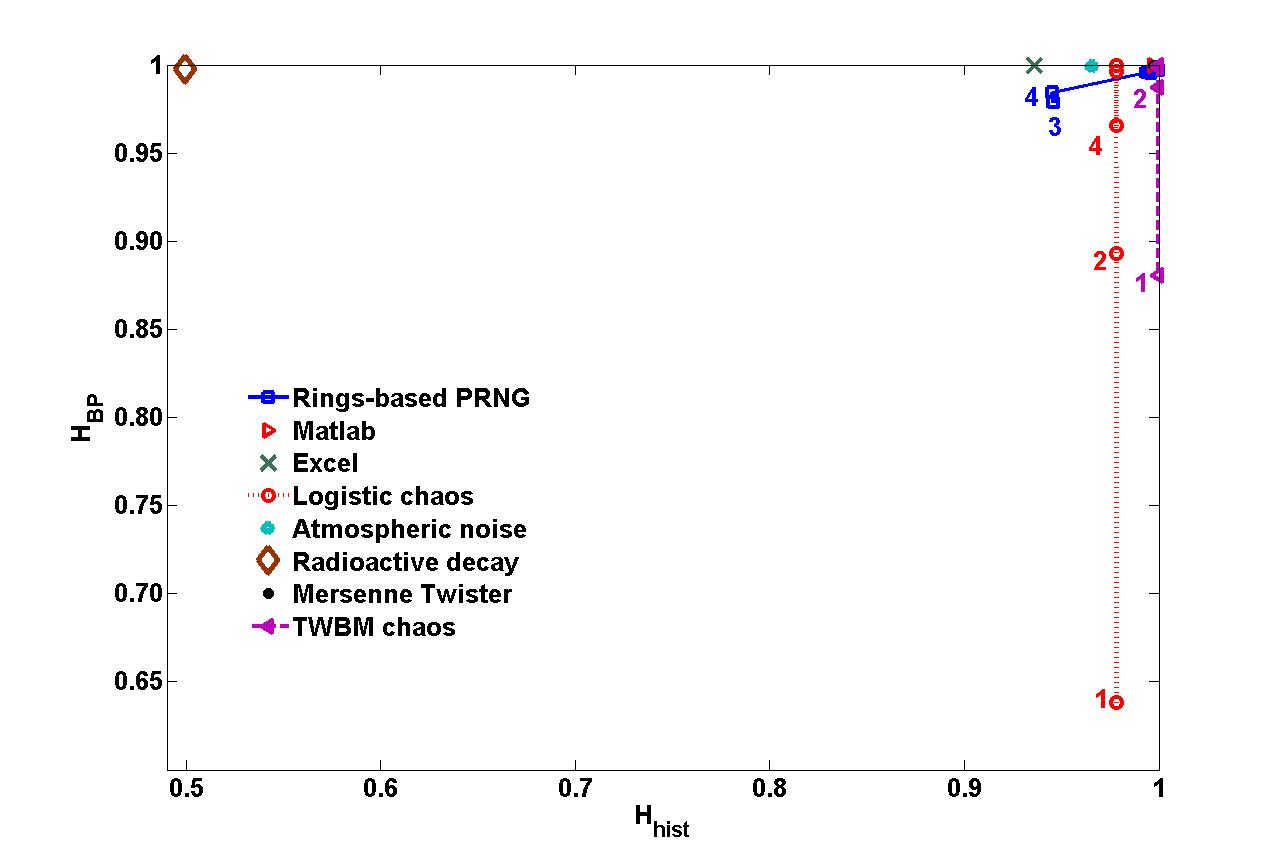
\includegraphics[ width=0.8\textwidth]{HhistvsHBP_t}
\caption{$H_{BP}$ vs $H_{hist}$ plane for several noises, numbers next to each square indicate the quantity of \emph{RO}s
used in the \emph{RO} based \emph{PRNG}. Numbers next to each point in the  chaotic sequences labeled \emph{Logistic}
and \emph{TWBM} indicate the number of iteration of the chaotic map (see the text for details).}
\label{fig:HBPvsHhis_all}
\end{center}
\end{figure*}
%=========================================

In the case of the \emph{RO}-based \emph{PRNG} sequences, numbers next to each square indicate the quantity of \emph{RO}s employed in that \emph{PRNG} (let us stress that the number of inverters is fixed to $3$). The dual entropy plane shows that  an increase in the number of \emph{RO}s improves both $H_{BP}$ and $H_{hist}$.

Fig. \ref{HhistvsHBP_zoom} is a zoom of Fig. \ref{fig:HBPvsHhis_all}  around the ideal point $(1,1)$.


%=========================================
 % FIGURA
\begin{figure*}
\begin{center}
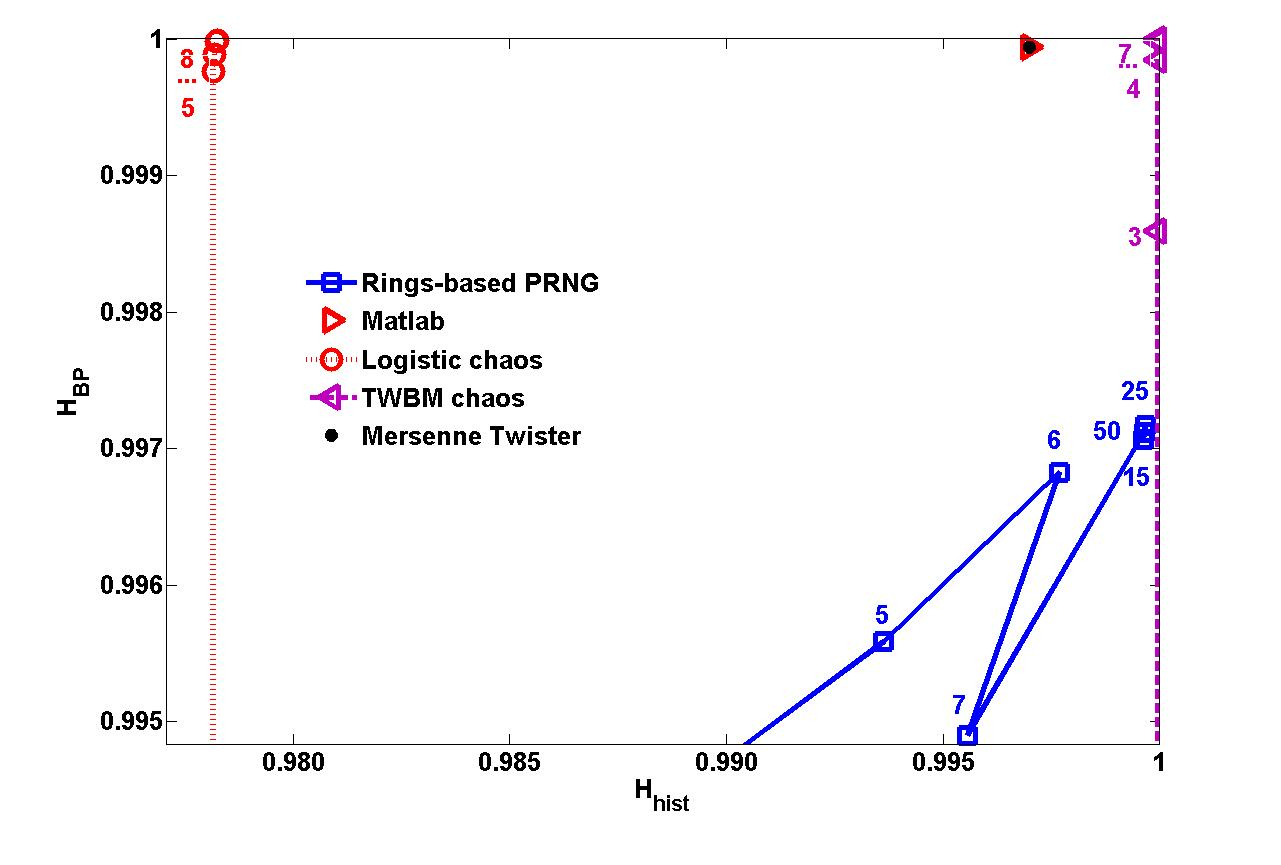
\includegraphics[ width=0.8\textwidth]{HhistvsHBP_z}
\caption{Zoom of Fig. \ref{fig:HBPvsHhis_all}  around the ideal point $(1,1)$ of the $H_{BP}$ vs $H_{hist}$ plane. Numbers next to each square indicate the number of \emph{RO}s used in that rings-based \emph{PRNG}. Numbers next to each point in the chaotic sequences indicate the number of iteration of the chaotic map.} \label{HhistvsHBP_zoom}
\end{center}
\end{figure*}
%=========================================

There, it is shown the evolution of the \emph{RO}-based \emph{PRNG} sequences when the quantity of \emph{RO}s increases from $5$ to $50$ (numbers next to each square). It can be seen that as the number of rings increases, data increase their mixture and also the histogram tends to be more uniform. So both properties are improved. Here a threshold in the number of rings can be determined, as the points saturate at about $(0.997,1)$, so this is the best \emph{PRNG} possible. Further, using more than $15$ \emph{RO}s presents no improvement.
As it was previously said, $H_{hist}$ quantifier detects the histogram variation of the sequence, and the $H_{BP}$ quantifier reflects the improvement in the mixing of data.
Finally, Mersenne Twister and Matlab sequences present identical value, ideal $H_{BP}$, and a high value of $H_{hist}$ nonetheless the histogram is not perfectly uniform (values are not equiprobable).

\section{Conclusiones}
\label{sec:conclusions}
\emph{RO}-based \emph{PRNG} implemented here has demonstrated to satisfactorily meet the statistical properties desired by a \emph{PRNG}. They are comparable of other used \emph{PRNG}s and in some cases they are better. They employs few resources of the device and they are simply to implement in a digital platform.

It was demonstrated that for these architectures of \emph{PRNG} the quantity of
\emph{RO}s establishes \emph{PRNG}'s statistical properties. It was seen that
for $15$ \emph{RO}s both output's statistical properties, histogram
and mixing, were almost ideal, making unnecessary the increase of the number of rings.

The dual entropy plane proposed here has demonstrated to satisfactorily discern between the \emph{PRNG}'s two main desired properties, the equiprobability among all possible values and the statistical independence between consecutive values. Thus, it allows to clearly see what needs to be improved in a given sequence.